\documentclass[12pt,a4paper]{article}
\usepackage[utf8]{inputenc}
\usepackage{amsmath}
\usepackage{amsfonts}
\usepackage{amssymb}
\usepackage{makeidx}
\usepackage{graphicx}
\usepackage[left=2cm,right=2cm,top=2cm,bottom=2cm]{geometry}

\begin{document}
\title{\textbf{Sistemas electronicos de interfaz\\EV 1.3. Circuitos de control de voltaje y corriente con tiristores\\Practica 3}}
\author{Angel Eraclio Briano Garcia\\Ing. Mecatronica\\Grado 4B}
\date{01 de noviembre del 2019}
\maketitle
\begin{figure}[h!]
\centering

\includegraphics[width=10cm]{UPCDLZMDG5783-logo.png} 
\end{figure}
\newpage

\section{Introducciòn}
En esta practica (Que ya es algo vieja) aprenderemos a utilizar 

\section{Objetivo}
Lograr hacer que el foco incandesente cambiara su intensidad modulando la misma con un potenciometro.

\section{Materiales}
Protoboard\\Resistencia de 1K\\Potenciometro de 500K\\Cables de protoboard\\Diac\\Triac\\Foco incandesente con clavija y base\\Laptop (Simulador a elegir)

\section{Desarrollo}
\textbf{1-} Como primera instancia de la practica, se procedera a simular el circuito para asi tener mas claro lo que se tiene que hacer y asi lograr ver errores antes de llegar a quemar alguno de nuestros componentes, el circuito en cuestiòn es el siguiente.
\begin{figure}[h!]
\centering
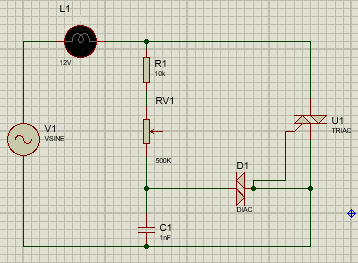
\includegraphics[width=8cm]{Practica3.jpg} 
\end{figure}

\textbf{2-} Una vez simulado se puede proceder a armarlo algo mas confiados ya que se vio anteriormente como es que puede llegar a reaccionar el circuito, claro en esta parte depende mas de como es que se le conecte asi que hacerlo con cuidado, en caso de duda preguntar a algun compañero o directamente con el asesor.
\newpage

\textbf{3-} Una vez ya armado y funcionando, se debera de colocar marcas en el potenciometro para asi tener mas claro en que momento de la perilla la luz de nuestro foco comienza a obtener intensidad y cuando se le ve mas tenue, en este caso solo obtuvimos tres medidas, baja, media y alta. En algunos de los casos de los demas compañeros llegaron a obtener hasta 4 resultados diferentes.

\section{Conclusiòn}
Para concluir con esta practica, cabe resaltar la importancia del tipo de capacitor que se utiliza, tambien el funcionamiento que se le puede dar al potenciometro como un regulador de intencidad en complemeto con los demas componentes.  

\end{document}